\documentclass[a4paper,12pt]{article}

\usepackage{graphicx}
\usepackage{tabu}
\usepackage{tikz}
\usepackage{amsmath}
\usepackage{amssymb}
\usepackage{pgfplots}

\begin{document}
\title{Unit XXVI Assignment II}
\author{Nathan Windisch}
\date{March 2017}
\maketitle
\pagenumbering{arabic}
\tableofcontents
\newpage

\section{Sequences and Series}
The following are answers to questions set for the first task.
\subsection{nth and 17th Terms}
Find a formula for the \textbf{nth} term of this sequence and find the \textbf{17th} term using your \textsc{nth} term formula. Also calculate the \textbf{sum of the first 17 terms of this sequence}.

If the squence is \texttt{-3, 1, 5, 9, 13 ...} then we know that the formula must start with \textsc{4x+[SOMETHING]} due to the fact that the difference between each number and the last is +4. Now we need to calculate what the other part of the formula is. Not figure this out, we must subtract a number from the first value to enable \textsc{4x} to line up with our current sequence. This means that we need to subtract \textsc{7} from all numbers in the current formula in order for them to be accurate with our sequence. This means that the other part of our formula is \textsc{-7}, meaning that the forumla thus far is \textsc{4x+-7} or, more simply, \textsc{4x-7}. Therefore, the \textsc{nth} term will be \textsc{4x-7}.

Now, we need to apply our new found formula to the extended system, meaning that the following occurs:

\[
  {1n..17n = -3, 1, 5, 9, 13, 17, 21, 25, 29, 33, 37, 41, 45, 49, 53, 57, 61}
\]

This means that the 17th term is \textsc{61}.

\newpage

\subsection{Sums to Terms and Infinity}
Find a formula for the \textbf{nth} term of this sequence and find the \textbf{10th} term using your \textsc{nth} term formula. Also calculate the \textbf{sum to the 5th term} and the \textbf{sum to infinity} of this sequence.

\subsubsection{nth Term}
If the seqence is \texttt{81, -27, 9, -3 ...} then we know that there will not be an easy solution to this problem. This is because there is no obvious correlation between these numbers. To solve this, we will need to find the difference between the first and the second number, which is \textsc{108}. The difference between the second and the third number is \textsc{36}, and the difference between \textsc{12}. From these numbers, we can tell that the difference between each number and the last one is

\[
  \frac{previousNumber}{3}
\]

Because of this, we can calculate that the first part of the formula is
\[
  a * r^{n-1}
\]

We know that the common ratio, which in this case is \texttt{r}, is
\[
  \frac{-1}{-3}
\]

This means that we can apply this to the current sequence, resulting in:

\[
  a * r^{n-1} = 81 * \frac{1}{3}^{n-1}
\]

\newpage

\subsubsection{10th Term}
Within this section, all I need to do is apply the \texttt{10th term} to the previously generated formula, as follows:

\[
  81 * -\frac{1}{3}^{10-1}
\]

We can condense this further, giving us:

\[
  81 * -\frac{1}{3}^{9}
\]

Now we merely need to calculate the right side of the equation:

\[
  81 * -\frac{1}{19683}
\]

And subtitute the \texttt{1} with \texttt{81} as it is a multiplication of the numerator.

\[
  -\frac{81}{19683}
\]

Now we just condense the equation:

\[
  -\frac{1}{243}
\]

\subsubsection{Sum to 5th Term}
The formula that we need to perform this equation is as follows:

\[
  S_n = \frac{a_1(r^n-1)}{r-1}
\]

In a similar fashion to the previous question, I shall now just substitute the algebraic numbers within the sample formula with my own data:

\[
  \frac{81(-\frac{1}{3}^5-1)}{-\frac{1}{3}-1}
\]

We can condense this down into the following equqation:

\[
  \frac{81(-0.004115226..-1)}{-1.\dot{3}}
\]

Now we just expand the brackets:

\[
  \frac{81 * -1.004115226..}{-1.\dot{3}}
\]

And finally we do the final calculation on the left side of the equation:

\[
  -\frac{81.\dot{3}}{1.\dot{3}}
\]

This gives us the final number of:

\[
  61
\]

\newpage

\subsubsection{Sum to Infinity}
To generate a \texttt{Sum to Infinity} you need to use the following formula:

\[
  S = \frac{a}{(1-r)}
\]

As in all the previous iterations of this question, I just need to substitute the formula with my own data, as follows:

\[
  \frac{81}{(1--\frac{1}{3})}
\]

Now we need to cancel out the negatives:

\[
  \frac{81}{(1+\frac{1}{3})}
\]

We can now combine the numbers on the bottom of the fraction together:

\[
  \frac{81}{(1+1\dot{3})}
\]

This gives us the final number of:

\[
  60.75
\]

\newpage

\subsection{Equations}
Find the solution to
\[
  \sum_{r=1}^6 (3r - 2r^2 + r^3)
\]

Substituting the Rs for 1s.
\[
  \sum_{r=1}^6 ((3 \times 1) - (2 \times 1^2) + (1^3))
\]

Substituting the Rs for 2s.
\[
  \sum_{r=2}^6 ((3 \times 2) - (2 \times 2^2) + (2^3))
\]

Substituting the Rs for 3s.
\[
  \sum_{r=3}^6 ((3 \times 3) - (2 \times 3^2) + (3^3))
\]

Substituting the Rs for 4s.
\[
  \sum_{r=4}^6 ((3 \times 4) - (2 \times 4^2) + (4^3))
\]

Substituting the Rs for 5s.
\[
  \sum_{r=5}^6 ((3 \times 5) - (2 \times 5^2) + (5^3))
\]

Substituting the Rs for 6s.
\[
  \sum_{r=6}^6 ((3 \times 6) - (2 \times 6^2) + (6^3))
\]

\newpage

Working out the brackets where R = 1.
\[
  \sum^6_{r=1} (3 - (2 \times 1) + 1)
\]

Working out the brackets where R = 2.
\[
  \sum^6_{r=2} (6 - (2 \times 4) + 8)
\]

Working out the brackets where R = 3.
\[
  \sum^6_{r=3} (9 - (2 \times 9) + 27)
\]

Working out the brackets where R = 4.
\[
  \sum^6_{r=4} (12 - (2 \times 16) + 64)
\]

Working out the brackets where R = 5.
\[
  \sum^6_{r=5} (15 - (2 \times 25) + 125)
\]

Working out the brackets where R = 6.
\[
  \sum^6_{r=6} (18 - (2 \times 36) + 216)
\]

\newpage

Final solution within the brackets where R = 1.
\[
  \sum^6_{r=1} (3 - 2 + 1)
\]

Final solution within the brackets where R = 2.
\[
  \sum^6_{r=2} (6 - 8 + 8)
\]

Final solution within the brackets where R = 3.
\[
  \sum^6_{r=3} (9 - 18 + 27)
\]

Final solution within the brackets where R = 4.
\[
  \sum^6_{r=4} (12 - 32 + 64)
\]

Final solution within the brackets where R = 5.
\[
  \sum^6_{r=5} (15 - 50 + 125)
\]

Final solution within the brackets where R = 6.
\[
  \sum^6_{r=6} (18 - 72 + 216)
\]

\newpage

Final solution without the brackets where R = 1.
\[
  \sum^6_{r=1} (2)
\]

Final solution without the brackets where R = 2.
\[
  \sum^6_{r=2} (6)
\]

Final solution without the brackets where R = 3.
\[
  \sum^6_{r=3} (18)
\]

Final solution without the brackets where R = 4.
\[
  \sum^6_{r=4} (44)
\]

Final solution without the brackets where R = 5.
\[
  \sum^6_{r=5} (90)
\]

Final solution without the brackets where R = 6.
\[
  \sum^6_{r=6} (162)
\]

\newpage

Therefore we need to add up all the numbers to get the final figure.
\[
  \sum (2 + 6 + 18 + 44 + 90 + 162)
\]

This means that the final answer is:
\[
  322
\]

\newpage

\subsection{Balls in Bags}

Five balls are in a bag, 3 are red and 2 are yellow. Once a ball is chosen at random the ball is put back into the bag and the bag is shaken well.

\begin{figure}[h!]
  \includegraphics[width=\linewidth]{probabilitytable.png}
  \caption{Probability Table.}
  \label{fig:chart1}
\end{figure}

\newpage

\subsubsection{What is the probability that a yellow ball is selected?}

The answer to the first question is
\[
  \frac{2}{5}
\]

This is because there is a total of five balls in the bag, and two of those are yellow meaning that there is a two in five chance of ever getting a yellow ball.

\subsubsection{What is the probability 2 yellow balls are selected consecutively?}

The answer to the second question is
\[
  \frac{4}{10}
\]

This is because there can be a maximum of 2 balls taken out if the answer is correct, and they both need to be yellow. Because of this, the chance of getting the first ball is two in five, as is the second.

\subsubsection{Draw a probability tree and use it to find the probability that a yellow ball is selected 4 times in a row.}

The answer to the third question is
\[
  \frac{16}{625}
\]

This is because 2 x 2 x 2 x 2 is 16 and 5 x 5 x 5 x 5 is 625. We multiply these numbers as the probabibility of getting one Yellow is two out of five, so therefore we need to multiply it by itself four times as we want to get the total value of all four balls being yellow.

\newpage

\subsection{Venn Diagrams}

\subsubsection{The Diagram}

\def\firstcircle{(0,0) circle (1.5cm)}
\def\secondcircle{(55:2cm) circle (1.5cm)}
\def\thirdcircle{(0:2cm) circle (1.5cm)}
\def\forthcircle{(5,0.5) circle (1.5cm)}

\begin{tikzpicture}
  \draw \firstcircle node[below] {$M$};
  \draw \secondcircle node [above] {$C$};
  \draw \thirdcircle node [below] {$E$};
  \draw \forthcircle node [below] {$N$};

  % Now we want to highlight the intersection of the first and the
  % second circle:

  \begin{scope}
    \fill[cyan] \firstcircle;
  \end{scope}

  \begin{scope}
    \fill[gray] \secondcircle;
  \end{scope}

  \begin{scope}
    \fill[teal] \thirdcircle;
  \end{scope}

  \begin{scope}
    \fill[olive] \forthcircle;
  \end{scope}

  \begin{scope}
    \clip \firstcircle;
    \fill[red] \secondcircle;
  \end{scope}

  \begin{scope}
    \clip \secondcircle;
    \fill[violet] \thirdcircle;
  \end{scope}

  \begin{scope}
    \clip \firstcircle;
    \fill[yellow] \thirdcircle;
  \end{scope}

  \begin{scope}
    \clip \firstcircle;
    \clip \secondcircle;
    \fill[green] \thirdcircle;
  \end{scope}
\end{tikzpicture}

In this Venn diagram, the:
\begin{enumerate}
  \item {\color{cyan}Cyan} part is for the students that only take Computer Science.
  \begin{itemize}
    \item This number is 70 students.
  \end{itemize}
  \item {\color{gray}Gray} part is for the students that only take Engineering.
  \begin{itemize}
    \item This number is 83 students.
  \end{itemize}
  \item {\color{teal}Teal} part is for the students that only take Mathematics.
  \begin{itemize}
    \item This number is 0 students.
  \end{itemize}
  \item {\color{olive}Olive} part is for the students that take none of the above.
  \begin{itemize}
    \item This number is 10 students.
  \end{itemize}
  \item {\color{yellow}Yellow} part is for the students that take both Computer Science and Mathematics.
  \begin{itemize}
    \item This number is 15 students.
  \end{itemize}
  \item {\color{violet}Violet} part is for the students that take both Engineering and Mathematics.
  \begin{itemize}
    \item This number is 12 students.
  \end{itemize}
  \item {\color{red}Red} part is for the students that take both Computer Science and Engineering.
  \begin{itemize}
    \item This number is 0 students.
  \end{itemize}
  \newpage
  \item {\color{green}Green} part is for the students that take all the subjects, Computer Science, Engineering and Mathematics.
  \begin{itemize}
    \item This number is 0 students.
  \end{itemize}
\end{enumerate}

\subsubsection{Probability: Computer Science but not Mathematics}

The total number of all of these students is

\[
  70 + 83 + 0 + 10 + 15 + 12 + 0 + 0 = 190
\]

This means that the probability of a random Computer Science student that does not take Mathematics is

\[
  \frac{70}{190}
\]

Which, similifed is:

\[
  \frac{35}{95}
\]

And similfying it even more makes:

\[
  \frac{7}{19}
\]

\subsubsection{Probability: Engineering with or without other subjects}

The total number of all of these students is:

\[
  70 + 83 + 0 + 10 + 15 + 12 + 0 + 0 = 190
\]

This means that the probability of a random Engineering student that either does or does not take another subject is:

\[
  \frac{83 + 12}{190}
\]

Which, similifed is:

\[
  \frac{95}{190}
\]

And similfying it even more makes:

\[
  \frac{1}{2}
\]

\newpage

\subsection{Betting Game}
A betting game involves one player throwing a six sided die to represent an attack and the other player throwing a four sided die to represent a defence.
\subsubsection{Draw a probability space diagram for this game.}
\begin{center}
  \setlength{\arrayrulewidth}{.05em}
  \begin{tabu}{|c|[2pt]c|c|c|c|c|c|}
      \hline
      + & 1 & 2 & 3 & 4 & 5 & 6  \\\tabucline[2pt]{-}
      1 & 2 & 3 & 4 & 5 & 6 & 7  \\\hline
      2 & 3 & 4 & 5 & 6 & 7 & 8  \\\hline
      3 & 4 & 5 & 6 & 7 & 8 & 9  \\\hline
      4 & 5 & 6 & 7 & 8 & 9 & 10 \\\hline
  \end{tabu}
\end{center}

\subsubsection{What is the most likely total score(s) from both dice?}
The most likely total score when both dice are thrown is 4, 5, 6 and 7 as they have an equal amount of percentage within the table.
\[
  \frac{4}{24}
\]
is the percentage for each of the four numbers. Simpilfied, this is
\[
  \frac{1}{6}\mbox{ or }1.\dot{6}
\]

\subsubsection{What is the least likely score(s) and why?}
The least likely total score when both dice are thrown is 2 and 10 as they have an equal amount of percentage within the table.
\[
  \frac{1}{24}
\]
is the percentage for each of the two numbers. This cannot be simplified as the previous fraction has the lowest common numerator.

\newpage

\section{Number Systems}
The following table needs to be completed and two more rows need to be added. The following is the original table.

\subsection{Tables}
\begin{center}
  \setlength{\arrayrulewidth}{.05em}
  \begin{tabu}{|c|[2pt]c|c|c|c|}
    \hline
      & Denary & Binary & Octal & Hexadecimal \\\tabucline[2pt]{-}
    a & 22     & -      & -     & 13          \\\hline
    b & -      & -      & 13    & -           \\\hline
    c & 41     & -      & -     & -           \\\hline
    d & -      & 10100  & -     & -           \\\hline
    e & -      & -      & 36    & -           \\\hline
    f & -      & -      & -     & 2A          \\\hline
    g & 271    & -      & -     & -           \\\hline
    h & -      & -      & -     & -           \\\hline
    i & -      & -      & -     & -           \\\hline
  \end{tabu}
\end{center}

The following is my updated version of the table.

\begin{center}
  \setlength{\arrayrulewidth}{.05em}
  \begin{tabu}{|c|[2pt]c|c|c|c|}
    \hline
      & Denary & Binary    & Octal & Hexadecimal \\\tabucline[2pt]{-}
    a & 22     & 10110     & 26    & 16          \\\hline
    b & 11     & 1011      & 13    & B           \\\hline
    c & 41     & 101001    & 51    & 29          \\\hline
    d & 14     & 10100     & 24    & 14          \\\hline
    e & 30     & 11110     & 36    & 1E          \\\hline
    f & 42     & 101010    & 52    & 2A          \\\hline
    g & 271    & 100001111 & 417   & 10F         \\\hline
    h & 135    & 100000111 & 207   & 87          \\\hline
    i & 87     & 101011    & 127   & 57          \\\hline
  \end{tabu}
\end{center}

\newpage

\section{Number System Calculations}
\subsection{Hexadecial Calculations}
\subsubsection{Hexadecimal Adition}
I need to add together two hexadecimal functions that are found within the previous table.
\[
  a + f = 22 + 42 = 64
\]
Within the previous equation I used the denary numbers for the $a$ and $f$ values, meaning that the output number was in denary.

Because of this, I had to convert the denary number, which was in Base10 into a hexadecimal number, which is in Base16.
\[
  64_{10} = 40_{16}
\]
As a result, we can conclude that:
\[
  a + f = 40
\]

\subsubsection{Hexadecimal Multiplication}
I need to multiply two hexadecimal functions together, which were found within the previous table.
\[
  g * f = 271 * 42 = 11382
\]
Within the previous equation I used the denary numbers for the $g$ and $f$ values, meaning that the output number was in denary.

Because of this, I had to convert the denary number, which was in Base10 into a hexadecimal number, which is in Base16.
\[
  11382_{10} = 2C76_{16}
\]
As a result, we can conclude that:
\[
  g * f = 2C76
\]

\newpage

\subsubsection{Hexadecimal Subtraction}
I need to subtract one hexadecimal value from another, which were found within the previous table.
\[
  f - b = 42 - 11 = 31
\]
Within the previous equation I used the denary numbers for the $f$ and $b$ values, meaning that the output number was in denary.

Because of this, I had to convert the denary number, which was in Base10 into a hexadecimal number, which is in Base16.
\[
  31_{10} = 1F_{16}
\]
As a result, we can conclude that:
\[
  f - b = 1F
\]

\newpage

\subsection{Octal Calculations}
  \subsubsection{Octal Addition}
    I need to add two octal functions together, which were found within the previous table.
    \[
      a + e = 22 + 30 = 52
    \]
    Within the previous equation I used the denary numbers for the $a$ and $e$ values, meaning that the output number was in denary.

    Because of this, I had to convert the denary number, which was in Base10 into a octal number, which is in Base8.
    \[
      52_{10} = 64_{8}
    \]
    As a result, we can conclude that:
    \[
      a - e = 64
    \]

  \subsubsection{Octal Subtraction}
    I need to subtract one octal value from another, which were found within the previous table.
    \[
      e - b = 30 - 11 = 19
    \]
    Within the previous equation I used the denary numbers for the $e$ and $b$ values, meaning that the output number was in denary.

    Because of this, I had to convert the denary number, which was in Base10 into an octal number, which is in Base8.
    \[
      19_{10} = 23_{8}
    \]
    As a result, we can conclude that:
    \[
      e - b = 23
    \]

\newpage

\subsection{Binary Calculations}
  \subsubsection{Binary Addition}
    I need to add two binary functions together, which were found within the previous table.
    \[
      a + d = 22 + 14 = 36
    \]
    Within the previous equation I used the denary numbers for the $a$ and $d$ values, meaning that the output number was in denary.

    Because of this, I had to convert the denary number, which was in Base10 into a binary number, which is in Base2.
    \[
      36_{10} = 100100_{2}
    \]
    As a result, we can conclude that:
    \[
      a + d = 100100
    \]

  \subsubsection{Binary Multiplication}
    I need to multiply two binary functions together, which were found within the previous table.
    \[
      a * d = 22 * 14 = 308
    \]
    Within the previous equation I used the denary numbers for the $a$ and $d$ values, meaning that the output number was in denary.

    Because of this, I had to convert the denary number, which was in Base10 into a binary number, which is in Base2.
    \[
      308_{10} = 100110100_{2}
    \]
    As a result, we can conclude that:
    \[
      a * d = 100110100
    \]

\newpage

\subsection{Additional Equations}
  I also have to perform two more additional equations of my own choice.
  \subsubsection{Hexadecimal Addition}
    I need to add together two hexadecimal functions that are found within the previous table.
    \[
      e + c = 30 + 41 = 71
    \]
    Within the previous equation I used the denary numbers for the $a$ and $f$ values, meaning that the output number was in denary.

    Because of this, I had to convert the denary number, which was in Base10 into a hexadecimal number, which is in Base16.
    \[
      71_{10} = 47_{16}
    \]
    As a result, we can conclude that:
    \[
      e + c = 47
    \]

  \subsubsection{Binary Subtraction}
    I need to subtract one binary value from another, which were found within the previous table.
    \[
      f - d = 42 - 14 = 28
    \]
    Within the previous equation I used the denary numbers for the $a$ and $d$ values, meaning that the output number was in denary.

    Because of this, I had to convert the denary number, which was in Base10 into a binary number, which is in Base2.
    \[
      28_{10} = 11100_{2}
    \]
    As a result, we can conclude that:
    \[
      f - d = 11100
    \]

\newpage

\section{Data Task}
  \subsection{Data}
    \subsubsection{Hypothesis}
      The data that I shall be collecting and working with free data that was generated by the \texttt{US Bureau of Labour Statistics}. The data is about the unemployment rate within the United States from 1948 to 2004, inclusive. The data is in the form of percentages and all people within the data are aged 16 or over.
      The data is over 30 years and has a percentage for each month. I shall be using this data to generate a mean, median of each year, by adding up all of the numbers within the set. I shall also use this data to determine averages.
      My hypothesis is that more people will be hired around December due to the need for more people as there are more roles to be filled due to the festivities.

    \subsubsection{Data Set}
      \setlength{\arrayrulewidth}{.05em}
      \begin{tabu}{|c|[2pt]c|c|c|c|c|c|c|c|c|c|c|c|c|}
        \hline
        Year & Jan & Feb & Mar & Apr & May & Jun & Jul & Aug & Sep & Oct & Nov & Dec & AVG \\\tabucline[2pt]{-}
        1994 & 6.6 & 6.6 & 6.5 & 6.4 & 6.1 & 6.1 & 6.1 & 6.0 & 5.9 & 5.8 & 5.6 & 5.5 & 6.1 \\\hline
        1995 & 5.6 & 5.4 & 5.4 & 5.8 & 5.6 & 5.6 & 5.7 & 5.7 & 5.6 & 5.5 & 5.6 & 5.6 & 5.6 \\\hline
        1996 & 5.6 & 5.5 & 5.5 & 5.6 & 5.6 & 5.3 & 5.5 & 5.1 & 5.2 & 5.2 & 5.4 & 5.4 & 5.4 \\\hline
        1997 & 5.3 & 5.2 & 5.2 & 5.1 & 4.9 & 5.0 & 4.9 & 4.8 & 4.9 & 4.7 & 4.6 & 4.7 & 4.5 \\\hline
        1998 & 4.6 & 4.6 & 4.7 & 4.3 & 4.4 & 4.5 & 4.5 & 4.5 & 4.6 & 4.5 & 4.4 & 4.4 & 4.5 \\\hline
        1999 & 4.3 & 4.4 & 4.2 & 4.3 & 4.2 & 4.3 & 4.3 & 4.2 & 4.2 & 4.1 & 4.1 & 4.0 & 4.2 \\\hline
        2000 & 4.0 & 4.1 & 4.0 & 3.8 & 4.0 & 4.0 & 4.0 & 4.1 & 4.0 & 3.9 & 3.9 & 3.9 & 3.9 \\\hline
        2001 & 4.2 & 4.2 & 4.3 & 4.4 & 4.3 & 4.5 & 4.6 & 4.9 & 5.0 & 5.4 & 5.6 & 5.7 & 4.8 \\\hline
        2002 & 5.6 & 5.7 & 5.7 & 5.9 & 5.8 & 5.8 & 5.8 & 5.7 & 5.7 & 5.7 & 5.9 & 6.0 & 5.8 \\\hline
        2003 & 5.8 & 5.9 & 5.8 & 6.0 & 6.1 & 6.1 & 6.2 & 6.1 & 6.1 & 6.0 & 5.9 & 5.7 & 5.9 \\\hline
        2004 & 5.6 & 5.6 & 5.7 & 5.6 & 5.6 & 5.6 & 5.5 & 5.4 & 5.4 & 5.5 & 5.4 & 5.5 & 5.5 \\\hline
      \end{tabu}

  \newpage

  \subsubsection{Frequency Diagram}
    %freqdiag
    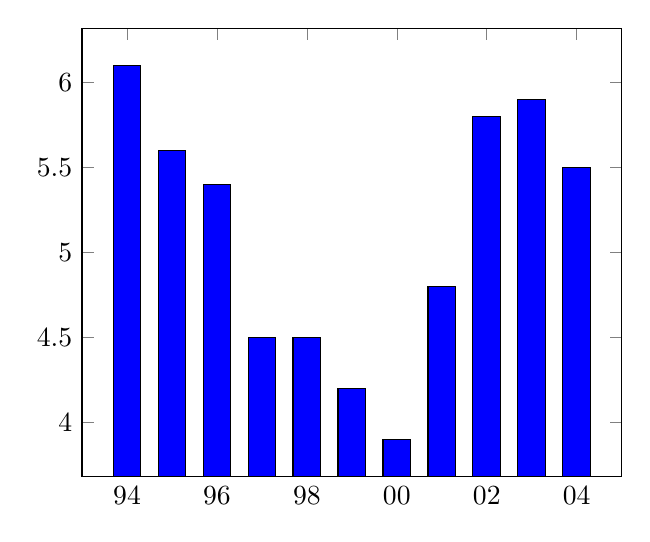
\begin{tikzpicture}
      \begin{axis}[
        symbolic x coords={94, 95, 96, 97, 98, 99, 00, 01, 02, 03, 04},
        xtick=,
        ]
        \addplot[ybar,fill=blue] coordinates {
          (94, 6.1)
          (95, 5.6)
          (96, 5.4)
          (97, 4.5)
          (98, 4.5)
          (99, 4.2)
          (00, 3.9)
          (01, 4.8)
          (02, 5.8)
          (03, 5.9)
          (04, 5.5)
        };
      \end{axis}
    \end{tikzpicture}

  In the above graph, the X axis is the year and the Y axis is the average unemployment rate percentage over the year.

  \subsubsection{Mean, Median and Mode}
    \paragraph{Mean}
      The Mean is the total of all of the numbers in the dataset, divided by the amount of numbers that are in the dataset. The total of all of the numbers within the dataset is 681.3, and the total amount of numbers within the dataset is 120 as there are 12 months over 10 years. Therefore, when we multiply the total of all the numbers in the dataset with the amount of data that there is we get:
      \textbf{681.3 * 120 = 81756}

      \paragraph{Median}
        The Median is the centre value within the dataset. This means that the middle months are June and July, and the middle years are 1998 and 1999. The result of this is that we need to get the values for both of those, and then work out an average. The unemployment percentage rate in June 1998 was 4.5, July 1998 was 4.5, June 1999 was 4.3 and July 1999 was 4.3. This means that the average all of these numbers is 4.4, as it is in the centre is all four of the numbers, due to there being only two unique numbers. The result of this is that the median is \textbf{5.4}.

      \paragraph{Mode}
        The mode is the value that is the most common number within the dataset. With the dataset that we are currently using, the most common number is \textbf{5.6}.

      \paragraph{Range}
        The range is the difference between the lowest number within the dataset and the highest number within the dataset. In our dataset, the lowest number is 3.8 and the highest number is 6.6, so the difference between these numbers is 2.8. This means that we have to add half of 2.8 to 3.8, meaning that the number in between the highest and lowest number is \textbf{5.2}.

      \paragraph{Interquartile Range}
        The Interquartile Range is a method of getting the variablility of a dataset. It works by dividing the data into quartiles, meaming that the dataset has been split into four equal parts, and the value of each of these parts are called the \textit{first}, \textit{second} and \textit{third quartiles}, or \textbf{Q1}. \textbf{Q2} and \textbf{Q3}, respectively.

  \newpage

  \subsubsection{Box Plot}
    \begin{figure}[h!]
      \includegraphics[width=\linewidth]{boxplot.jpg}
      \caption{A box plot generated from the data.}
      \label{fig:chart2}
    \end{figure}

    The values within the box plot are as follows:
    \[
      Population Size: 132
    \]
    \[
      Q1 = 4.425
    \]
    \[
      Q3 = 5.7
    \]
    \[
      IQ Range = 1.275
    \]
    \[
      Outliers: None
    \]

    \paragraph{Varience}
      The variance is a way to measure how far a set of numbers is spread out.

      To calculate the variance, we first need to get the mean value. After this we need to subtract it from each piece of data that we have. Then we square all the numbers that we have thus far, to ensure that they are positive. Now we need to add them all together and divide this number by the total number of values in the dataset. This results in the variance for your dataset.

  \subsubsection{Conclusion}
    Judging from the information I have gathered, it seems people look at their watches on average 11 times a day. This would make sense, as the information I gathered was in college, which means people would need to check the time often to make sure they were going to get to the right lessons on time. I suspect that because of this, the results would be different in a different work environment, such as an office or a catering job.

\newpage

\section{Recursion}
  %define recursion
  In computing, a recursive method is a piece of self-contained code that will call upon its self repeatedly. These are often used in algorithms such as specialized sorting algorithms, that are designed to go through large amounts of data quickly. For example, a Non-Recursive algorithm would be a loop that would go through each element of data and check if it is the data that it is looking for, if it was, the code would return the value and stop the loop. This means that if the piece of data happens to be at the beginning of the data set, the code is very quick. But if the data is at the end of the data set, it can take a long time to get to the correct piece of data, as it must check each piece of data in order.
  A Recursive Sorting algorithm would be a Binary Search. This would check the middle value of the data set, if it was not the value it was looking for, it would recursively call its self to check for the middle value of the 2 halves of the data set. The code would keep doing this until it found the piece of data it was looking for. This method is efficient for large data sets.

\section{Number Systems}
  %define binary
  Binary is the simplest form of data transfer, and is used by computers to transfer information. Binary is represented by 0’s and 1’s, and different combinations can mean different things. Binary can also be interpreted differently, so the same combination of 0’s and 1’s can mean one thing, but can also be interpreted to mean another. One use of binary is to represent characters, such as numbers and letters, there are different ways of doing so, such as ASCII and Unicode. This is how Binary can be converted to ASCII.

  %define hex
  Hexadecimal is a shorthand way of representing binary. It is easier to read and understand for a person, so it is often used instead of binary in places where a person might need to right the information. For example, Hex is used to represent colours on computer systems, the colours are split between Red, Blue and Green, and sometimes a transparency value. For example, FFFFFF converts to pure white, while 000000 is pure black.

  %define octal
  Octal is not often used in computer systems anymore, as computers are now based on multiples of 4 rather than 3, which means hexadecimal is used more often. However, Octal is still used on Unix system permissions as there are 3 groups, User, Group, and Others. And its file permissions are set to read, write, and execute, and as an Octal character can represent 3 Binary characters, it makes it very well suited for this task.
\end{document}
